\documentclass[11pt]{article}
\usepackage[pdftex]{graphicx}
\usepackage[explicit]{titlesec}
\usepackage[OT1]{fontenc}
\usepackage[most]{tcolorbox}
\usepackage[final]{pdfpages}
\usepackage[colorlinks=true, urlcolor=cyan, hyperfootnotes=false]{hyperref}
\usepackage{fullpage, graphicx, psfrag, url, caption, authblk, amsfonts, amsmath, amssymb, float, fancyhdr, multicol, cmbright, xcolor, amsthm, gensymb, physics}

\fancypagestyle{pages}{
	%Headers
	\fancyhead[L]{Physics 7A, Summer 2024 \\ Section 103}
	%\fancyhead[C]{\thepage}
	\fancyhead[R]{Discussion 1 \\ June 17}
\renewcommand{\headrulewidth}{0pt}
	%Footers
	%\fancyfoot[L]{}
	\fancyfoot[C]{}
	\fancyfoot[R]{\thepage}
\renewcommand{\footrulewidth}{0pt}
}

\newcommand\blfootnote[1]{
    \begingroup
    \renewcommand\thefootnote{}\footnote{#1}
    \addtocounter{footnote}{-1}
    \endgroup
}

\newcommand{\fig}[4]{
    \begin{figure}[H]
        \centering
        \includegraphics[scale={#3}, angle={#4}]{#1}
        \caption{#2}
        \label{exp4fit}
    \end{figure}
}

\newtheoremstyle{gangnamstyle}{}{}{}{}{\sffamily\bfseries}{.}{ }{}
\tcolorboxenvironment{definition}{boxrule=0pt,boxsep=0pt,colback={blue!10},left=8pt,right=8pt,enhanced jigsaw, borderline west={2pt}{0pt}{blue},sharp corners,before skip=10pt,after skip=10pt,breakable}
\tcolorboxenvironment{example}{boxrule=0pt,boxsep=0pt,colback={orange!10},left=8pt,right=8pt,enhanced jigsaw, borderline west={2pt}{0pt}{orange},sharp corners,before skip=10pt,after skip=10pt,breakable}
\tcolorboxenvironment{problem}{boxrule=0pt,boxsep=0pt,colback={cyan!10},left=8pt,right=8pt,enhanced jigsaw, borderline west={2pt}{0pt}{cyan},sharp corners,before skip=10pt,after skip=10pt,breakable}
\theoremstyle{gangnamstyle}{\newtheorem{definition}{Definition}[]}
\theoremstyle{gangnamstyle}{\newtheorem{example}{Example}[]}
\theoremstyle{gangnamstyle}{\newtheorem{problem}{Problem}[]}

\headheight=0pt
\footskip=0pt
\setlength{\oddsidemargin}{0 in}
\setlength{\evensidemargin}{0 in}
\setlength{\topmargin}{-0.5 in}
\setlength{\textwidth}{6.5 in}
\setlength{\textheight}{8.5 in}
\setlength{\headsep}{0.75 in}
\setlength{\parindent}{0 in}
\setlength{\parskip}{0.1 in}

\begin{document}
\normalfont
\pagestyle{pages}

% Begin Document

\begin{center}
\vspace{3in}
{\Large Discussion 1 } \\ [0.05in]
Math Review, Preliminary Physics \\ [-0.5in]
\end{center}

\section*{Topics}
Calculus and Trigonometry, Units and Dimensions, Order of Magnitude

\section{Math Review}

\textbf{1.} Find the first and second derivatives of the following functions. \\
$A$, $k$, $n$ are constants. Assume $n \geq 2$ or $n \leq -1$. 
\begin{flalign*}
& f(x) = Ax^n & 
\end{flalign*}
\begin{flalign*}
& f(x) = A\cos(kx) & 
\end{flalign*}
\begin{flalign*}
& f(x) = A\sin(kx) & 
\end{flalign*}
\begin{flalign*}
& f(x) = Ae^{kx} & 
\end{flalign*}
\begin{flalign*}
& f(x) = Ae^{-kx} & 
\end{flalign*}

\textbf{2.} Use the chain rule to find the derivative of $f(x) = \sin(x^n)$. \\

\textbf{3.} Use the quotient rule to find the derivative of $f(x) = \tan(kx)$. \\
Hint: $\tan(\theta) = \frac{\sin(\theta)}{\cos(\theta)}$ \\

\textbf{4.} For some constant $k$, \\
If $f'(x) = kf(x)$, what could $f$ be? \\

If $f'(x) = -kf(x)$, what could $f$ be? \\

If $f''(x) = kf(x)$, what could $f$ be? \\

If $f''(x) = -kf(x)$, what could $f$ be? \\

\textbf{5.} \textit{Zimba, Force and Motion, Problem 2.8 (Next two pages)}. 

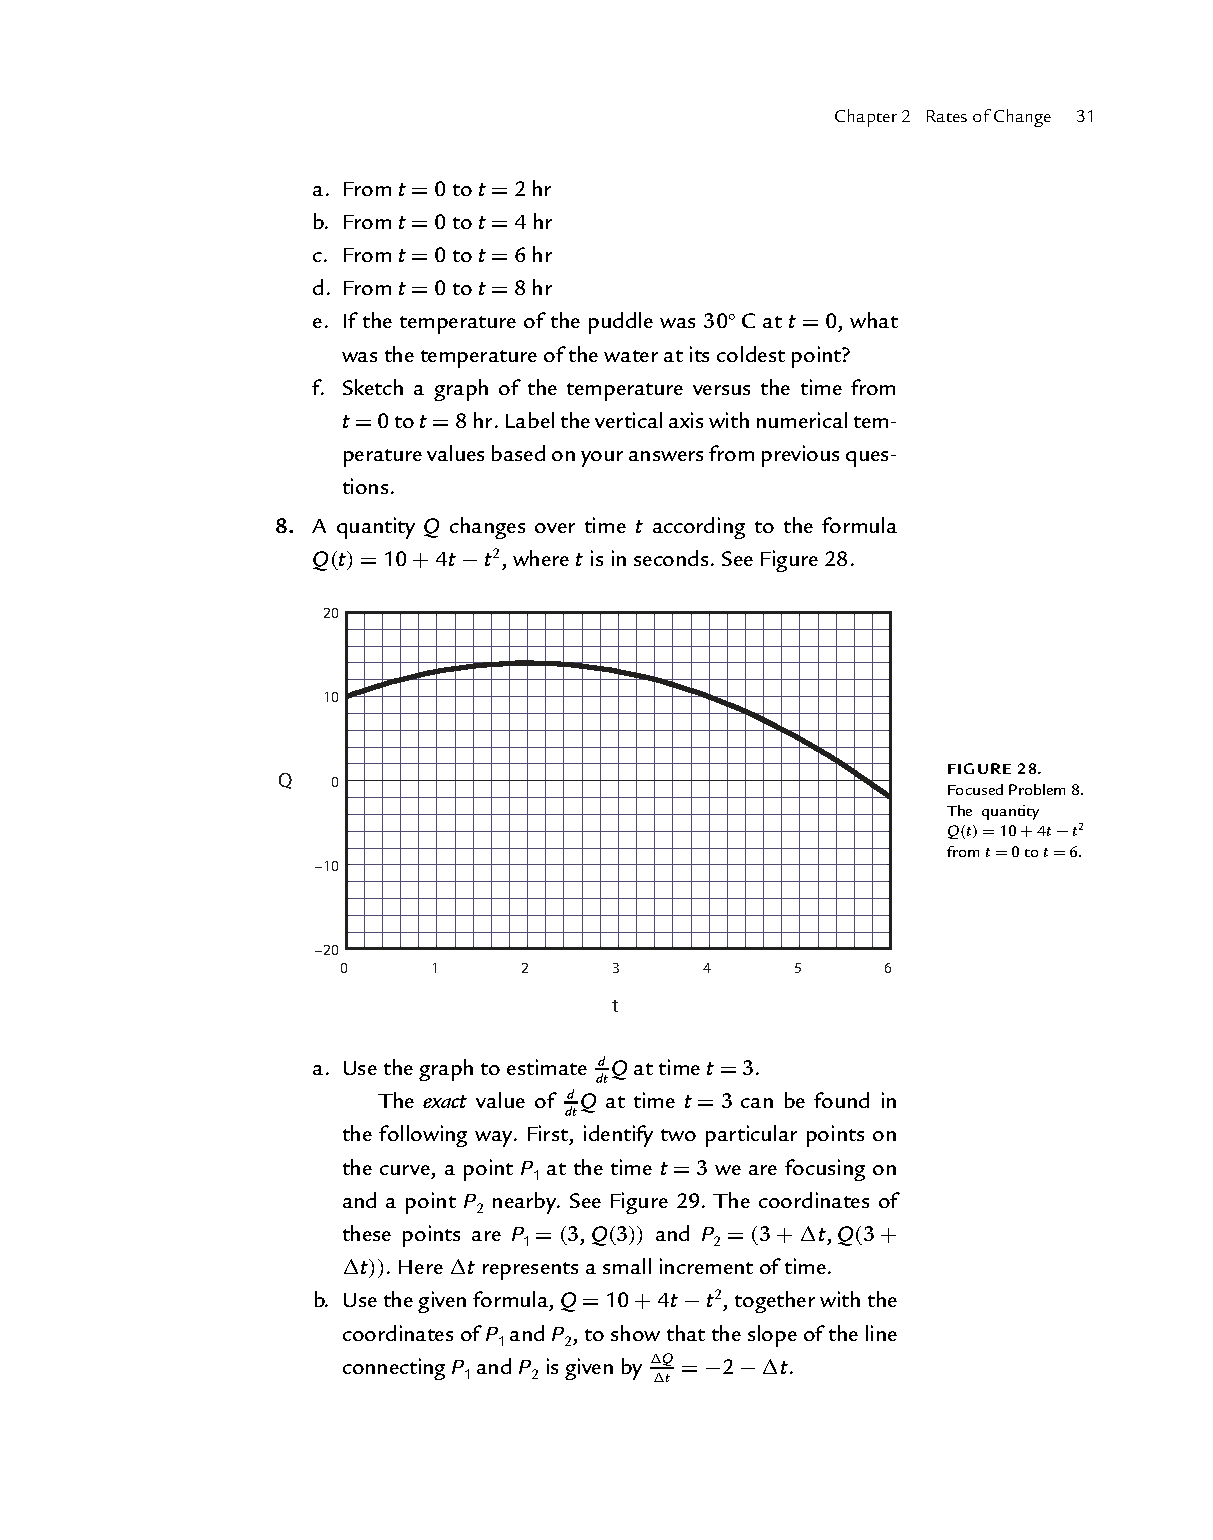
\includepdf[pages=-]{figs/0617/fm.pdf}

\section{Dimensional Analysis}

\textbf{1.} \textit{Giancoli, Physics for Scientists and Engineers, Problem 1.55} \\
The speed $v$ of an object is given by the equation $v = At^3 + Bt$, where $t$ refers to time (seconds). \\
(a) What are the dimensions of $A$ and $B$? \\
(b) What are the SI units for the constants $A$ and $B$? \\
\vspace{0.5 in}

\textbf{2.} \textit{Giancoli, Physics for Scientists and Engineers, Problem 1.56} \\
Three students derive the following equations in which $x$ refers to distance traveled, $v$ the speed, $a$ the acceleration ($m/s^2$), $t$ the time, and the subscript zero ($0$) means a quantity at time $t = 0$. Here are their equations: \\
(a) $x = vt^2 + 2at$ \\
(b) $x = v_0t + \frac{1}{2}at^2$ \\
(c) $x = v_0t + 2at^2$ \\
Which of these could possibly be correct according to a dimensional check, and why?
\vspace{0.5 in}

\textbf{3.} A person throws a ball with speed $v$ off a cliff of height $h$, launched at an angle $\theta$ of her choosing. It accelerates downward with constant acceleration $g$ due to gravity. Assuming that one of the following is the correct expression for the maximum horizontal distance the ball can travel before it hits the ground, using what you know about dimensional analysis and limiting cases, which is correct, and why? Try to surmise the correct answer without actually solving for the trajectory. \\
(a) $\frac{vh}{g}$ \\

(b) $\frac{gh^2}{v^2}$ \\

(c) $\frac{v^2}{g}$ \\

(d) $\sqrt{\frac{v^2h}{g}}$ \\

(e) $\frac{v^2}{g}\sqrt{1 + \frac{2gh}{v^2}}$ \\

(f) $\frac{v^2 / g}{1 - \frac{2gh}{v^2}}$ \\

\end{document}
